\ylDisplay{Värvitilgad} % Ülesande nimi
{Tundmatu autor} % Autor
{piirkonnavoor} % Voor
{2009} % Aasta
{P 1} % Ülesande nr.
{1} % Raskustase
{
% Teema: Võnkumine

\ifStatement
Ühtlaselt ja sirgjooneliselt liikuva horisontaalse laua kohal on kaks paigalseisvat düüsi, millest tilgub lauale värvi. Värvitilgad langevad samast düüsist vvõrdsete ajavahemike järel. Joonisel on kujutatud teatud osa lauast värvitilkade jälgedega (täpid $A$, $B$, $C$, $D$). Mitu korda erinevad tilkade langemise sagedused (ajaühikus langenud tilkade arv) erinevatest düüsidest?
\begin{center}
	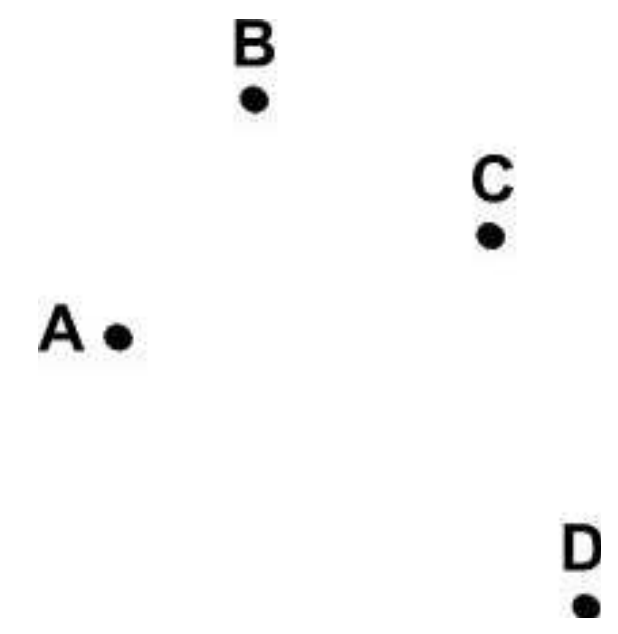
\includegraphics[width=0.5\linewidth]{2009-v2p-01-yl.PNG}
\end{center}
\fi

\ifHint
Laua sirgjoonelise liikumise tõottu peavad ühest ja samast düüsist langevate tilkade jäljed asetsema ühel sirgel, erinevate düüside jaoks peavad need sirged olema paralleelsed.
\fi

\ifSolution
Laua sirgjoonelise liikumise tõottu peavad ühest ja samast düüsist langevate tilkade jäljed asetsema ühel sirgel, erinevate düüside jaoks peavad need sirged olema paralleelsed. See jätab vaid võimaluse, et täpid $A$ ja $D$ pärinevad ühest ja $B$ ning $C$ teisest düüsist. \\
Langegu tilgad düüsidest vastavalt sagedustega $f_1$ ja $f_2$. Siis 
\begin{center}
$\mid AD \mid \cdot f_1 = \mid BC \mid \cdot f_2 = v$,
\end{center}
kus $v$ on laua liikumise kiirus ja $ \mid AD \mid$ ning $\mid BC \mid$ vastavate lõikude pikkused. Siit $\frac{f_2}{f_1} = \frac{\mid AD\mid}{\mid BC \mid}$. Mõõtes lõikude pikkused joniselt saame $\frac{f_2}{f_1} = 2$. \\
Vastus: tilkade langemise sagedused erinevad $2$ korda.
\fi
}